% Dans l'introduction, on présente le problème étudié et les buts
% poursuivis. L'introduction permet de faire connaître le cadre de la
% recherche et d'en préciser le domaine d'application. Elle fournit
% les précisions nécessaires en ce qui concerne le contexte de
% réalisation de la recherche, l'approche envisagée, l'évolution de
% la réalisation. En fait, l'introduction présente au lecteur ce
% qu'il doit savoir pour comprendre la recherche et en connaître la
% portée.

\Chapter{INTRODUCTION}\label{sec:Introduction}  % 10-12 lignes pour introduire le sujet.

\\
Support d'acrobatie entraînant le corps de l'utilisateur dans un mouvement de rotation, mais pouvant aussi être manipulée par ce dernier, la roue Cyr se trouve à mi-chemin entre les disciplines acrobatique, d'équilibrisme et de manipulation d'objet. La réalisation de figures acrobatiques repose sur l'équilibre dynamique entre la roue et le corps de l'utilisateur. Ce dernier module le rythme et la force qu'il applique à la roue en fonction de sa masse, son inertie, sa géométrie. La popularité croissante des matériaux composites pour la fabrication d'équipement de cirque comme les mats ou les portiques éveille la curiosité de la communauté circassienne sur les possibilités nouvelles qu'une roue Cyr en composites apporterait. L'enjeu est double: le procédé de fabrication offrant un éventail de possibilités géométriques inaccessibles avec les métaux ainsi qu'un choix de propriétés mécaniques plus varié, c'est une opportunité d'optimiser des mouvements déjà existants mais aussi d'inventer de nouvelles figures avec une roue Cyr faite d'un matériau dont les propriétés élastiques permettent, par exemple, de sauter avec la roue.
%%
%%  CONCEPTS DE BASE / BASIC CONCEPTS
%%
\section{Définitions et concepts de base}  % environ 2-3 pages

\subsection{Définitions}
\paragraph{Circassien(ne):} relatif au cirque 
\paragraph{Agrès de cirque:} équipement nécessaire à la pratique d'une discipline circassienne. Exemples: la roue Cyr, le trapèze, le tissu aérien, les cannes d'équilibre, le mat chinois...
\paragraph{Disque d'Euler:} disque ayant un mouvement de rotation similaire à celui d'une pièce qu'on fait tourner sur une surface plane. Lorsque son mouvement entre en phase terminale sa vitesse de rotation augmente de façon impressionnante, ce qui lui a valu de devenir un jouet éducatif, mais aussi de faire l'objet de nombreuses publications scientifiques. Son mouvement est similaire à un des mouvements caractéristiques de la roue Cyr.


\subsection{Historique de la roue Cyr}
La roue Cyr que l'on retrouve dans les spectacles de cirque contemporains doit son  nom à Daniel Cyr, qui fabriqua sa première roue en 1996 \cite{Inertie}. A cette dernière, faite en une seule pièce d'acier recouverte d'un revêtement en PVC, succéda rapidement  une roue Cyr démontable en plusieurs parties. La première apparition marquante de la roue Cyr sur la scène circassienne eut lieu en 1998 dans un spectacle du Cirque Eloize, dont Daniel Cyr est le co-fondateur. Une médaille d'argent remportée en 2003 par ce dernier au Festival Mondial du Cirque de Demain acheva d'asseoir la popularité de ce nouvel agrès dans le secteur du cirque, mais également en tant que sport.\\
Cependant l'idée d'une roue à la géométrie torique dont le diamètre avoisine la taille humaine est bien antérieure à la création de Daniel Cyr \cite{Inertiehist,gymmedia,howstuffwork}. En effet, plusieurs agrès d'apparence similaire à celle de la roue Cyr sont apparus du côté de l'Allemagne dès le début du vingtième siècle. On remarquera en particulier l'Einrefen, inventé en 1930 par Adalbert von Rekowski, qui diffère de la roue Cyr par des poignées intérieures pour les mains et les pieds (figure \ref{fig:cyrhelga}). \\

\begin{figure}[h]
\centering
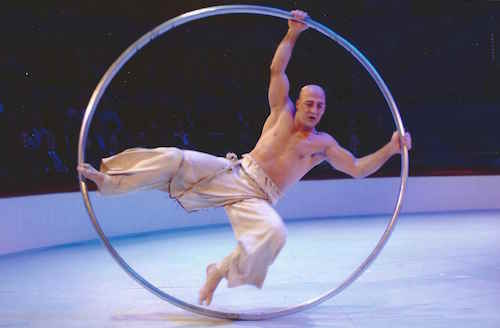
\includegraphics[width=200]{images_autres/danielcyr2003.jpeg}
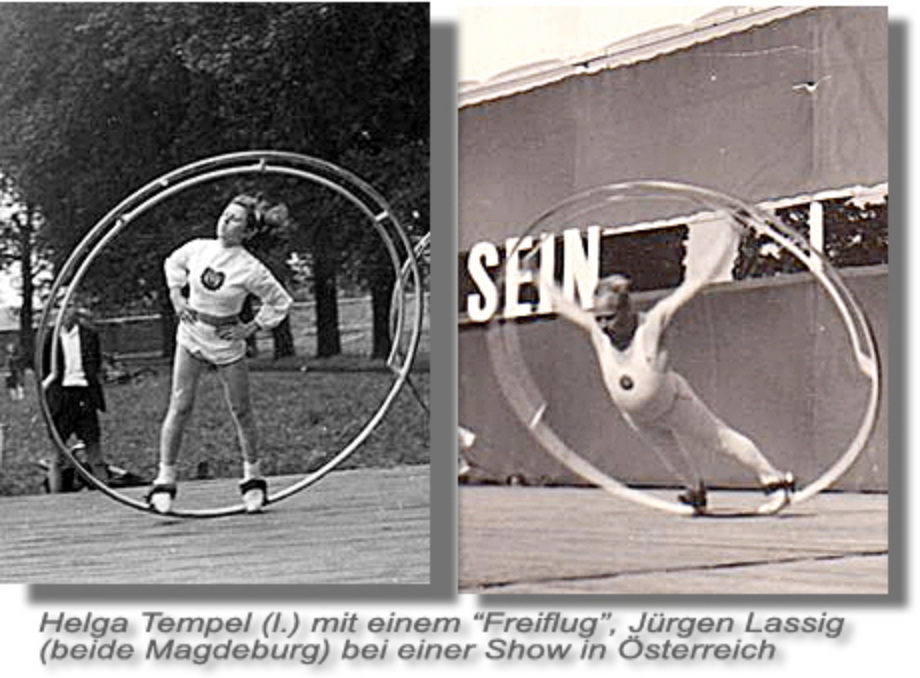
\includegraphics[width=200]{images_autres/helga1950.png}
\caption{Daniel Cyr au 24e festival mondial de demain en 2003 \cite{danielcyr} (gauche) et la gymnaste Helga Tempel sur l'Einrefen en 1950 \cite{gymmedia}) (droite).}
\label{fig:cyrhelga}
\end{figure}


Depuis, la roue Cyr continue d'évoluer, comme le montrent les agrès hybrides conçus en dérivant le concept de la roue Cyr pour créer de nouvelles possibilités acrobatiques (figure \ref{fig:cyrhyb}). Les procédés de fabrication se sont eux aussi affinés \cite{corbin}, et les roues Cyr lumineuses programmables ont vu le jour.\\
La fabrication en matériaux composites se présente aujourd'hui comme l'étape suivante dans l'évolution de l'agrès.

\begin{figure}[h]
\centering
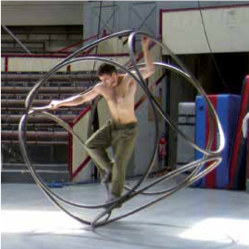
\includegraphics[width=120]{images_autres/hyb1.png}
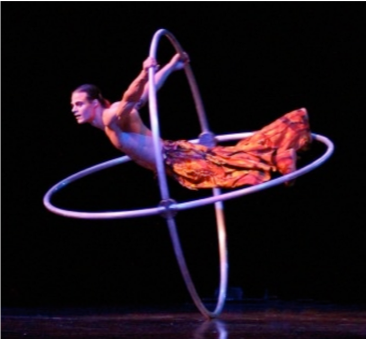
\includegraphics[width=130]{images_autres/hyb2.png}
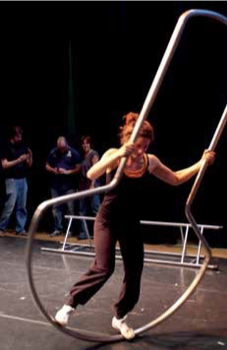
\includegraphics[width=80]{images_autres/hyb3.png}
\caption{Agrès de cirque dérivés de la roue Cyr \cite{Fedec2011}.}
\label{fig:cyrhyb}
\end{figure}

\subsection{Les figures de roue Cyr}
Nous présentons ici les figures de roue Cyr constituant la base principale de la discipline. Ces dernières, ainsi que d'autres figures plus avancées sont détaillées dans le manuel de la FEDEC \cite{Fedec2011}
\subsubsection{La valse (ou pas de base)}
Le corps est positionné de façon symétrique, avec bras et jambes chacun inclinés à 45\degree de la verticale. L'utilisateur initie la rotation d'une poussée du pied puis accompagne le mouvement de la roue en utilisant le transfert de son poids, tirant et poussant successivement la roue dans le sens de la rotation.\\
Ce mouvement se décline en plusieurs variations : par exemple un lâcher de pied, qui avec un arc de cercle de la jambe devient un arabesque. Il s'exécute aussi à une seule main, les mains croisées, en serrant et croisant les jambes ou en les écartant jusqu'au grand écart latéral. Il est aussi possible de placer un pied sur la roue au niveau de la tête, en grand écart facial. D'autres variantes jouent avec la position du corps : de profil, dans le plan de la roue, arqué vers l'intérieur, tendu vers l'extérieur...



\subsubsection{Les tours}
Dissociation du mouvement : la roue tourne mais pas le corps. Ce type de figure s'exécute en effectuant un demi-tour, un tour complet, ou même un tour en suspension avec l'utilisateur suspendu à la roue par une main.

\subsubsection{Les vrilles}
Dissociation inverse : le corps tourne dans le référentiel de la roue. De même ce type de figure se décline de la demi vrille à la vrille complète en suspension.

\subsubsection{Les suspensions}
Comme l'indique le nom, les pieds ne sont pas sur la roue. On peut par exemple exécuter la valse en suspension, sans les pieds, ou simplement prendre de l'élan puis lâcher les pieds et adopter une position groupée en tournant sur place, ce qui a pour effet d'augmenter la vitesse de rotation. Il est possible de se suspendre par une ou deux mains, par les coudes, les bras tendus ou fléchis. La suspension est la base de la figure du Superman: corps gainé, jambes tendues vers l'arrière.

\subsubsection{Le drapeau}
La roue n'est tenue que par la main et le pied d'un même côté. La rotation est alimentée en poussant et tirant avec la main et le pied restants, tout en tendant puis groupant successivement la main et le pied lâchés.

\subsubsection{Les sauts}
La roue tourne sur elle même, l'utilisateur saute et prend appui comme il le souhaite, bras tendus, pliés, ou même en position assise sur la roue. Il maintient sa position pour quelques tours et peut ensuite atterrir sur le sol ou directement sur la roue.

\subsubsection{Le corner ou inclinaison horizontale}
L'utilisateur se décale sur un côté de la roue jambes serrées, prend appui jambes fléchies puis plonge vers le sol, jambes tendues : le corps se retrouve en position horizontale pour un demi tour. Cette figure peut se réaliser en lâchant un bras, un pied, ou un bras et un pied simultanément.

\subsubsection{Le saut de mains}
L'utilisateur pousse la roue vers le sol avec une main, accompagne le renversement avec son poids, ouvre les doigts quand sa main arrive au niveau du sol puis la tire au dessus de sa tête et la pousse avec ses jambes afin de revenir à l'endroit. Cette figure s'exécute en avant, en arrière, en position de profil, à une jambe.

\subsubsection{La roue}
La roue roule sur sa tranche et l'utilisateur entretient le mouvement au moyen de transferts de poids. On peut enchaîner plusieurs roues le long d'une trajectoire circulaire ou rectiligne. Il est possible de la combiner avec d'autres figures ou changements de direction et d'enchaîner ainsi les roues dans des sens différents.

\subsubsection{La pièce}
Ce mouvement est semblable à la rotation d'une pièce de monnaie dans la phase terminale du mouvement. L'utilisateur, gainé, ouvre successivement les doigts pour ne pas les écraser lorsque ses mains arrivent au niveau du sol, et transfère son poids pour accompagner le mouvement et l'alimenter aussi longtemps qu'il le souhaite. Cette figure peut s'exécuter à différentes hauteurs du sol, plus la pièce est basse, plus la vitesse sera élevée. On peut aussi la réaliser à l'envers, le corps arqué (pièce dorsale).

\begin{figure}[h]
\centering
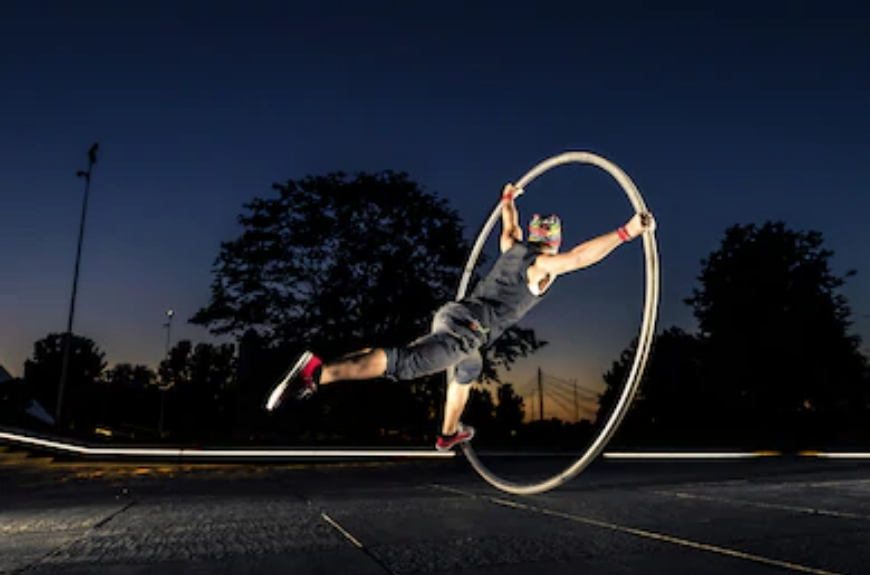
\includegraphics[width=200]{images_autres/valse.png}
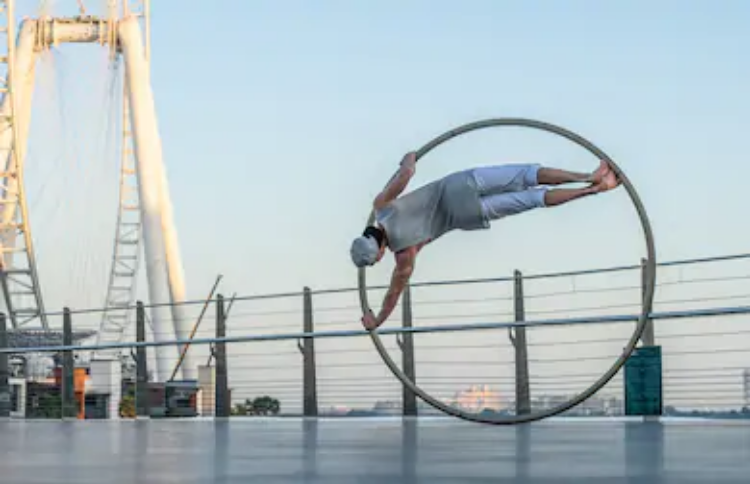
\includegraphics[width=210]{images_autres/corner.png}
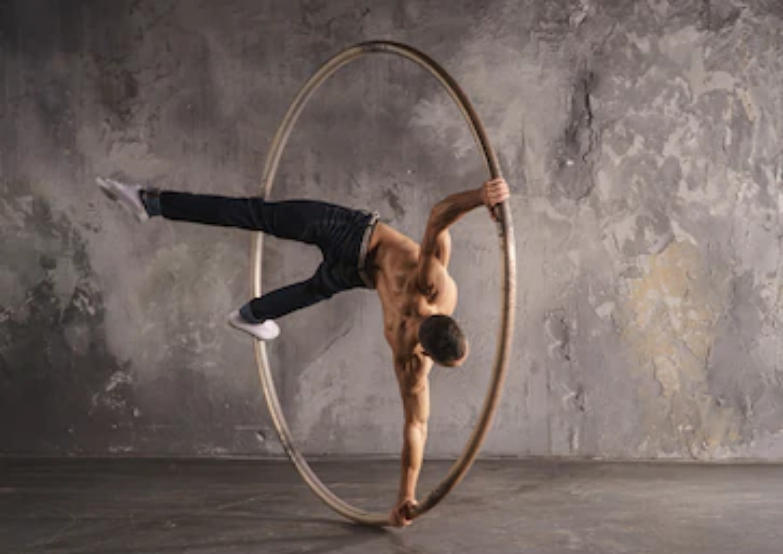
\includegraphics[width=200]{images_autres/handspring.png}
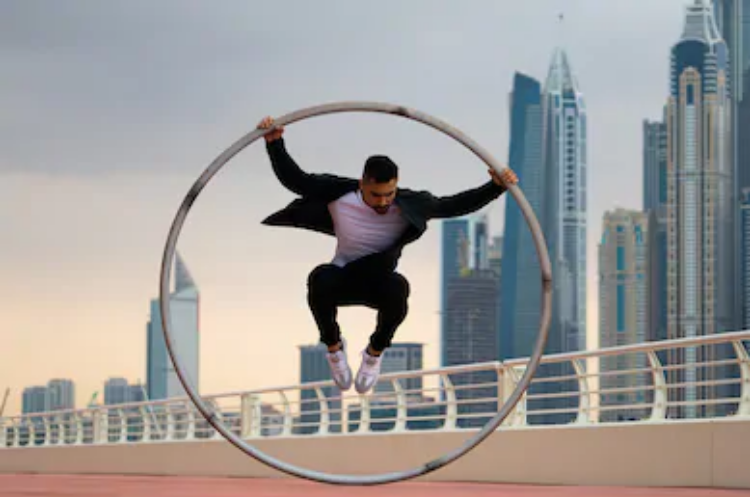
\includegraphics[width=210]{images_autres/suspension.png}
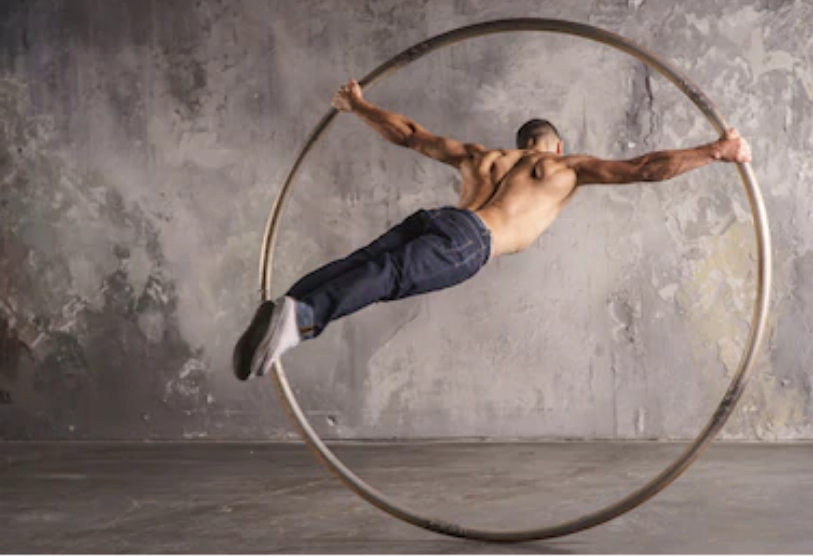
\includegraphics[width=200]{images_autres/superman.png}
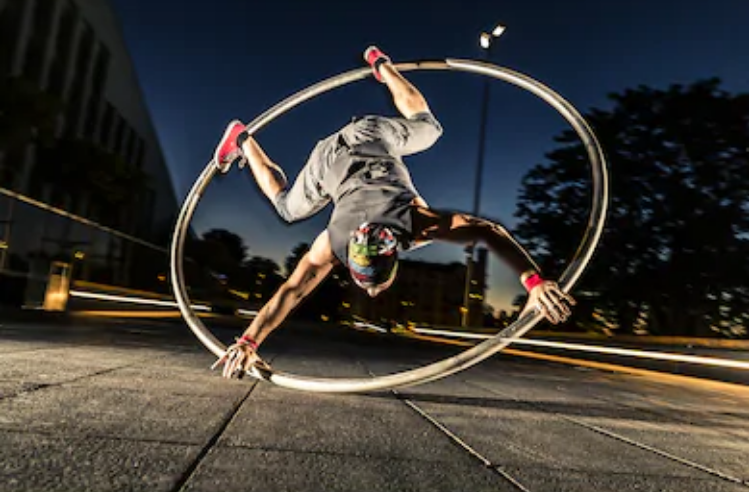
\includegraphics[width=210]{images_autres/piece.png}
\caption{Quelques figures de roue Cyr  \cite{shutterstock}. De gauche à droite: valse avec lâcher de pied, corner, saut de main, suspension, superman, pièce.}
\label{fig:figures}
\end{figure}

\clearpage

%%
%lt% anément eELEMENTt chent la roue simuS DE LA PROBLEMATIQUE
%%
\section{Problématique}  % environ 3 pages
La création d'une roue Cyr en matériaux composites enrichira la discipline de nouvelles figures et possibilités scéniques grâce à ses propriétés différentes de celles des roues Cyr classiques en métal. Ce projet se trouve au carrefour de la science, de la technique acrobatique et de l'art. Ceci nécessite de réunir des expertises issues de ces différents domaines, couplés à des moyens de fabrication adéquats. La problématique peut se découper selon les trois étapes clés du projet.

\subsection{Conception}
Il s'agit de déterminer quels paramètres parmi les propriétés mécaniques du matériau et la géométrie de la roue Cyr influencent les mouvements de cette dernière, puis de caractériser cette influence quantitativement. \\ 
A cet effet des modèles théoriques de deux mouvements caractéristiques ont été développés:
\begin{itemize}
    \item Le saut, la possibilité d’intégrer des sauts aux figures de roue Cyr déjà existante étant une des lignes directrices du projet. La roue est compressée par l'exercice d'une force verticale dont l’axe coïncide avec son diamètre, puis relâchée. Une part de l’énergie élastique stockée est convertie en saut. 
    \item Le mouvement correspondant à celui d’une pièce de monnaie qui roule sur sa tranche en décrivant des cercles, puis entre en phase terminale avant de tomber à plat sur le sol.
\end{itemize}

En se basant sur chacun des modèles théoriques correspondants, l’objectif est de déterminer séparément les paramètres géométriques et mécaniques qui :
\begin{itemize}
    \item  permettent à l’utilisateur de sauter le plus haut possible avec la roue.
    \item permettent d’optimiser le mouvement similaire à celui de la pièce de monnaie décrit ci-dessus en termes de stabilité dynamique.
    \item conduisent au meilleur compromis entre les deux réponses aux questions précédentes.
\end{itemize}


Parallèlement, il est nécessaire d’étudier les contraintes et déformations dans la roue afin d'anticiper les potentielles situations d'écoulement et de flambement et de les prendre en compte dans l'étape de conception.

\subsection{Fabrication}
Il s’agit de compléter l’étude théorique issue de la phase de conception par une utilisation adaptée de l’impression 3D. En utilisant les technologies existantes et disponibles pour le projet, comment imprimer un tore d’un diamètre avoisinant les deux mètres ? Comment assurer des propriétés conformes à celles déterminées par les modèles théoriques établis au préalable ? 

\begin{figure}[htb]
\centering
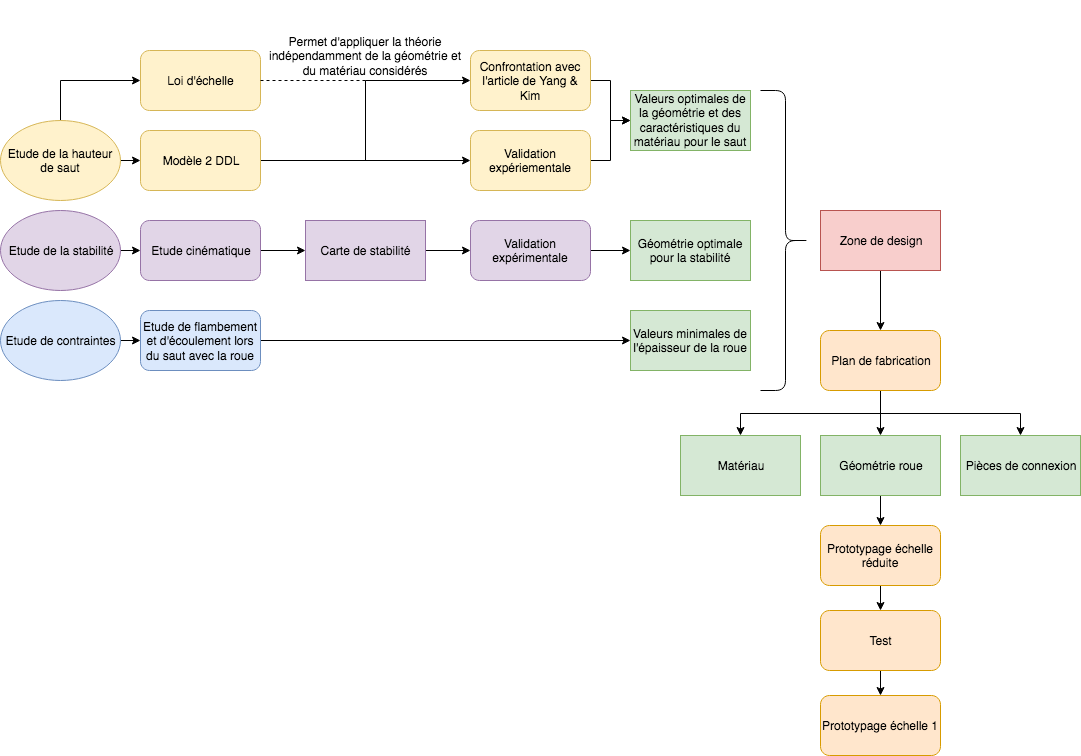
\includegraphics[width=7in]{images_autres/flowchart.png}
\caption{Flowchart résumant les étapes de conception et de fabrication de la roue.}
\label{fig:flowchart}
\end{figure}

\subsection{Tests}
Malgré la popularité du sujet au sein de la communauté circassienne, la roue en matériaux composites ne figure pas dans l'offre des fabricants d’équipement de cirque. Cela s'explique en partie par la difficulté à estimer concrètement ce qu’apporterait une telle roue Cyr et donc si les adeptes de la discipline seraient prêts à l'acquérir pour un prix supérieur à ceux des roues métalliques. Leur fabrication nécessite un investissement qui ne peut être engagé sans avoir de certitude sur sa rentabilité. Avec le prototype obtenu à l'issue de l'étape de fabrication, un phase de recherche artistique sera menée en collaboration avec des artistes de cirque. Les nouvelles possibilités introduites par une roue Cyr composite seront ainsi mises en évidence, aussi bien en termes d'acrobatie que de jeu de scène. Les fabricants seront ainsi en mesure d'évaluer si une véritable demande peut exister.\\
En outre, plusieurs artistes de roue Cyr ont déjà tenté d'approcher ces nouvelles possibilités, avec des roues Cyr fabriquées de manière artisanale dans des matériaux plus légers ou plus flexibles que les métaux (par exemple une roue Cyr en osier a été fabriquée par des élèves au Centre National des Arts du Cirque (CNAC) en France)
cependant ces projets d'expérimentation n'ont pu être menés à terme, les roues se retrouvant rapidement endommagées et hors service. Fournir un prototype fonctionnel et solide permettra à ces artistes de continuer d'approfondir leur recherche avec une sécurité accrue.

% On veut éviter que la figure et le tableau soient placés au-delà de la section courante.
\FloatBarrier


%%
%% OBJECTIFS DE RECHERCHE / RESEARCH OBJECTIVES
%%
\section{Objectifs de recherche}  % 0.5 page
\subsection{Objectif global}
L'objectif global de ce projet de recherche est de parvenir à la conception d’un prototype de roue Cyr optimisée grâce aux matériaux composites et à l'impression 3D, puis de tester avec des artistes les nouvelles possibilités offertes par cet agrès.

\subsection{Objectifs spécifiques}
Les objectifs spécifiques du projet sont les suivants:
\begin{itemize}
    \item Caractériser expérimentalement et théoriquement l’influence des propriétés mécaniques et de la géométrie sur le comportement dynamique de la roue Cyr
    \item Définir un matériau composite haute performance optimisé pour la roue Cyr
    \item Définir et mettre en oeuvre un procédé d'impression 3D adapté à nos problématiques
    \item Imprimer un prototype à partir du matériau choisi
    \item Conclure le projet par des sessions de recherche artistique autour du nouvel agrès
\end{itemize}


%%
%% PLAN DU MEMOIRE / THESIS OUTLINE
%%
\section{Plan du mémoire}  % 0.5 page
Ce mémoire s'organise en 5 chapitres. Le deuxième chapitre est constitué d'une revue de littérature centrée sur la roue Cyr, recensant les publications traitant de systèmes s'en rapprochant par leurs formes et leurs mouvements. Le chapitre trois expose une modélisation du saut d'une roue Cyr et sa validation expérimentale. Le chapitre quatre étudie la stabilité dynamique du mouvement de rotation d'une roue Cyr. Le chapitre cinq traite de la fabrication et du procédé d'impression 3D mis en oeuvre.